\documentclass[11pt,a4paper]{article}
\usepackage[utf8]{inputenc}
\usepackage[spanish]{babel}
\usepackage{amsmath}
\usepackage{amsfonts}
\usepackage{amssymb}
\usepackage{graphicx}
\usepackage[left=2cm,right=2cm,top=2cm,bottom=2cm]{geometry}
\usepackage{listings}
\usepackage[hidelinks]{hyperref}
\usepackage{lscape}
\usepackage{rotating}
\usepackage{pdflscape}

\lstset{
basicstyle=\ttfamily,
frame=single,
language=SQL,
tabsize=2,
showstringspaces=false,
literate=%
    {á}{{\'a}}1
    {é}{{\'e}}1
    {è}{{\`e}}1
    {í}{{\'i}}1
    {ó}{{\'o}}1
    {ú}{{\'u}}1
}

\begin{document}

\begin{titlepage}
	\title{{\Huge \textbf{Práctica 5 - Bases de Datos 2}}}
	\author{
	  Hayk Kocharyan\\
	  757715@unizar.es
	  \and
	  Juan José Tambo Tambo\\
	  755742@unizar.es
	  \and
	  Pedro Tamargo Allué\\
	  758267@unizar.es
	  \and
	  Jesús Villacampa Sagaste\\
	  755739@unizar.es
	}
	\date{\today}
	
	\clearpage\maketitle
	\thispagestyle{empty}
	\tableofcontents
	\listoffigures
\end{titlepage}

\section{Esfuerzos invertidos}

\begin{itemize}
\item Hayk:
	\begin{itemize}
	\item Instalación de Hadoop y HBase: 4 horas
	\item Implementación del código de Logistica.java: 3 horas
	\item Implementación del código de Validacion.java: 1 hora 
	\item Memoria: 2 horas
	\end{itemize}
\item Juan José:
	\begin{itemize}
	\item Implementación del código de Logistica.java: 3 horas
	\item Implementación del código de Validacion.java: 1 hora
	\end{itemize}
\item Pedro:
	\begin{itemize}
	\item  Instalación de Hadoop y HBase: 4 horas
	\item  Implementación del código de Logistica.java: 3 horas
	\item  Depuración de código de Logistica.java: 3 horas
	\item Implementación del código de Validacion.java: 1 hora
	\item Memoria: 3 horas
	\end{itemize}
\item Jesús:
	\begin{itemize}
	\item  Implementación del código de Logistica.java: 3 horas
	\item Implementación del código de Validacion.java: 1 hora
	\item Memoria: 1 hora
	\end{itemize}
\end{itemize}

\section{Instalación de Hadoop y HBase}

Para la instalación de \emph{Hadoop} y \emph{HBase} se han seguido los tutoriales disponibles en sus respectivas páginas oficiales. Se va a utilizar una máquina con \emph{SO Ubuntu 18.04}. \\
En el caso de \emph{Apache Hadoop} se ha procedido a configurar un servidor ssh para acceder a la propia máquina sin contraseña, utilizando una clave pública. Se puede instalar el servidor utilizando la órden:

\begin{lstlisting}
sudo apt update && sudo apt -y install openssh-server
\end{lstlisting}

Se va a proceder a crear e instalar una clave \emph{RSA} pública en nuestra máquina con el comando:

\begin{lstlisting}
cd ~/.ssh		  # Nos situamos en el directorio .ssh
ssh-keygen		# Creación de los ficheros de clave pública y privada
cat <id_rsa.pub >>authorized_keys
\end{lstlisting}

Tras esta configuración podremos acceder vía \emph{SSH} a la máquina sin contraseña mediante el comando:

\begin{lstlisting}
ssh localhost
\end{lstlisting}

\subsection{Apache Hadoop}

Después de la configuración técnica de la máquina se va a proceder a instalar \emph{Hadoop 3.2.1}. Se ejecutarán los siguientes comandos:

\begin{lstlisting}
wget http://apache.uvigo.es/hadoop/common/hadoop-3.2.1/		\
	hadoop-3.2.1.tar.gz
tar -xzvf hadoop-3.2.1.tar.gz
# Exportamos al PATH
export PATH="$PATH:$PWD/hadoop-3.2.1/bin:$PWD/hadoop-3.2.1/sbin" 
cd hadoop-3.2.1
\end{lstlisting}

Una vez se han descomprimido los ficheros se va a proceder a modificar los ficheros de configuración. Estos ficheros se encuentran en el directorio \emph{./etc/hadoop/}.\\
En el fichero \emph{hadoop-env.sh} se va a establecer la variable de entorno \emph{JAVA\_{}HOME}, para ello se insertarán las siguientes líneas:

\begin{lstlisting}
# set to the root of your Java installation
export JAVA_HOME=/usr/lib/jvm/java-8-openjdk-amd64
# Establecer el directorio raíz de Java
\end{lstlisting}

Se van a proceder a modificar los ficheros \emph{core-site.xml} y \emph{hdfs-site.xml}. En el primero, se va a modificar el contenido por el siguiente:

\begin{lstlisting}
<configuration>
    <property>
        <name>fs.defaultFS</name>
        <value>hdfs://localhost:9000</value>
    </property>
</configuration>
\end{lstlisting}

En el segundo fichero se va a modificar su contenido por el siguiente:

\begin{lstlisting}
<configuration>
    <property>
        <name>dfs.replication</name>
        <value>1</value>
    </property>
</configuration>
\end{lstlisting}

Tras la configuración de los ficheros se va a proceder a formatear el sistema de ficheros, para ello se va a proceder a ejecutar el siguiente comando:

\begin{lstlisting}
hdfs namenode -format
\end{lstlisting}

Tras esto, se habrá instalado \emph{Apache Hadoop}, no obstante faltará crear al usuario que interactuará con el sistema de ficheros distribuidos. Ejecutaremos los siguientes comandos:

\begin{lstlisting}
start-dfs.sh
hdfs dfs -mkdir -p /user/$LOGNAME
\end{lstlisting}

Para la configuración de \emph{YARN}, se va a proceder a parar todos los servicios (\texttt{stop-all.sh}) y a modificar los ficheros de configuración situados en \emph{./etc/hadoop/}. En el fichero \emph{mapred-site.xml} se establecerá el siguiente contenido:

\begin{lstlisting}
<configuration>
    <property>
        <name>mapreduce.framework.name</name>
        <value>yarn</value>
    </property>
    <property>
        <name>mapreduce.application.classpath</name>
        <value>$HADOOP_MAPRED_HOME/share/hadoop/mapreduce/*:		\
        		$HADOOP_MAPRED_HOME/share/hadoop/mapreduce/lib/*</value>
    </property>
</configuration>
\end{lstlisting}

Y en el fichero \emph{yarn-site.xml} se establecerá el siguiente contenido:

\begin{lstlisting}
<configuration>
    <property>
        <name>yarn.nodemanager.aux-services</name>
        <value>mapreduce_shuffle</value>
    </property>
    <property>
        <name>yarn.nodemanager.env-whitelist</name>
        <value>JAVA_HOME,HADOOP_COMMON_HOME,HADOOP_HDFS_HOME,	\
        		HADOOP_CONF_DIR,	CLASSPATH_PREPEND_DISTCACHE,		\
        		HADOOP_YARN_HOME,HADOOP_MAPRED_HOME</value>
    </property>
</configuration>
\end{lstlisting}

Se va a proceder a iniciar \emph{Hadoop} de nuevo, para ello se va a utilizar el siguiente comando:

\begin{lstlisting}
start-all.sh
\end{lstlisting}

\subsection{Apache HBase}

Para la instalación de \emph{Apache HBase 1.4.13} se va a proceder a descargar los binarios desde su página oficial utilizando los comandos:

\begin{lstlisting}
wget http://apache.uvigo.es/hbase/1.4.13/hbase-1.4.13-bin.tar.gz
tar -xzvf hbase-1.4.13-bin.tar.gz
# Exportamos la carpeta al path
export PATH="$PATH:$PWD/hbase-1.4.13/bin" 
cd hbase-1.4.13
\end{lstlisting}

Lo primero se va a proceder a modificar los ficheros de configuración situados en \emph{./conf}. En primer lugar modificaremos el fichero \emph{hbase-env.sh}, añadiremos las siguientes líneas:

\begin{lstlisting}
# Set environment variables here.
# The java implementation to use.
export JAVA_HOME=/usr/lib/jvm/java-8-openjdk-amd64
# Establecer el directorio raíz de Java
\end{lstlisting}

Ahora se va a proceder a modificar el fichero \emph{hbase-site.xml} modificando su contenido y añadiendo lo siguiente:

\begin{lstlisting}
<property>
  <name>hbase.cluster.distributed</name>
  <value>true</value>
</property>
<property>
  <name>hbase.rootdir</name>
  <value>hdfs://localhost:9000/hbase</value>
</property>
\end{lstlisting}

Tras esto, se va a proceder a ejecutar \emph{HBase}, para ello (con \emph{Hadoop} iniciado) se utilizará el comando:

\begin{lstlisting}
start-hbase.sh
\end{lstlisting}

Si se quiere acceder a hbase utilizando un prompt interactivo se puede utilizar el comando:

\begin{lstlisting}
hbase shell
\end{lstlisting}

\section{Pseudo-código de las funciones map y reduce utilizadas}

Para la adaptación del algoritmo de descenso de gradiente en \emph{Hadoop} se ha dividido el algoritmo proporcionado en el enunciado (Figura \ref{fig:pseudoenunciado}) en uno equivalente utilizando las funcionalidades de \emph{Map-Reduce} disponibles en \emph{Hadoop}.

La función \emph{map} se encargaría de emitir para cada clave $j$ el valor de cada uno de sus $n$ sumandos.\\
De esta manera la función \emph{reduce} se encargará de realizar ese sumatorio de $n$ sumandos y será una vez se haya completado la tarea de cálculo del vector gradiente cuando se hará el ajuste de los parámetros $\theta_{act}$.\\
De esta manera el pseudocódigo de las funciones mencionadas anteriormente quedará de la sieguiente manera:

\begin{lstlisting}
function map(key:clave1, value:valor1) {
	// clave1 se corresponde con el identificador del cliente a evaluar.
	// valor1 contiene toda la información asociada al cliente.
	// Hallamos el producto escalar 
	var prod_Esc = thetasAct * value[caracteristicas]
	// Calculamos yi en función de value[cliclass] es A o B
	var yi = if (value[cliclass] == A) then 0 else 1
	// Para cada caracteristica (indice, valor) de
	// value[caracteristicas] emitimos
	foreach (j,valor) in value[caracteristicas] do
		emit(j, (yi - g(prod_Esc))*valor )
	end
}
\end{lstlisting}

\begin{lstlisting}
function reduce(key:clave2, value:valor2) {
	// clave2 se corresponde con el identificador de
	// la caracteristica a evaluar.
	// valor2 contiene la lista de sumandos de la caracteristica j.
	// Hallamos el sumatorio
	emit(key, sum(value))
}
\end{lstlisting}


\label{listing:enunciado}

\section{Más cosas necesarias}

\section{Conclusiones sobre Hadoop y HBase}

\newpage
\section{Anexo 1: Figuras}

\begin{figure}[h!]
\centering
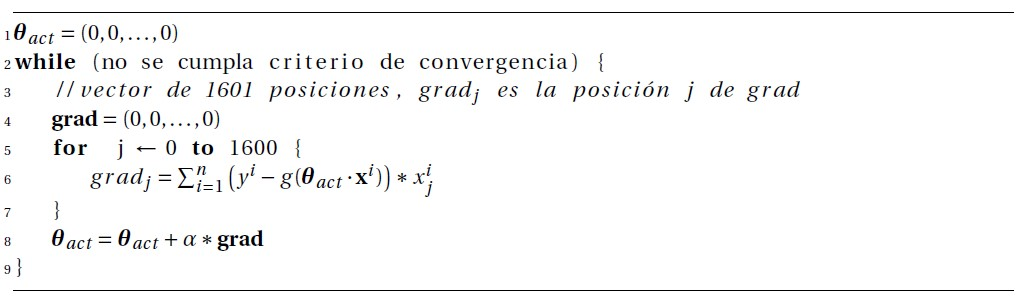
\includegraphics[scale=0.75]{images/pseudocodigo_enunciado.jpg}
\caption{Pseudocódigo proporcionado en el enunciado de la práctica}
\label{fig:pseudoenunciado}
\end{figure}


\end{document}